\documentclass[
	% -- opções da classe memoir --
	12pt,				% tamanho da fonte
	% openright,			% capítulos começam em pág ímpar (insere página vazia caso preciso)
    oneside,			% para impressão somente frente. Oposto a twoside (frente e verso)
	a4paper,			% tamanho do papel. 
	% -- opções da classe abntex2 --
	%chapter=TITLE,		% títulos de capítulos convertidos em letras maiúsculas
	%section=TITLE,		% títulos de seções convertidos em letras maiúsculas
	%subsection=TITLE,	% títulos de subseções convertidos em letras maiúsculas
	%subsubsection=TITLE,% títulos de subsubseções convertidos em letras maiúsculas
	% -- opções do pacote babel --
	english,			% idioma adicional para hifenização
	%french,				% idioma adicional para hifenização
	%spanish,			% idioma adicional para hifenização
	brazil,				% o último idioma é o principal do documento
	]{abntex2}


% ---
% PACOTES
% ---

% ---
% Pacotes fundamentais 
% ---
\usepackage{cmap}				% Mapear caracteres especiais no PDF
\usepackage{lmodern}			% Usa a fonte Latin Modern
%\usepackage{helvet}			% Usa a fonte helvet(ARIAL)
%\usepackage{pslatex}			
\usepackage[T1]{fontenc}		% Selecao de codigos de fonte.
\usepackage[utf8]{inputenc}		% Codificacao do documento (conversão automática dos acentos)
\usepackage{indentfirst}		% Indenta o primeiro parágrafo de cada seção.
\usepackage{color}				% Controle das cores
\usepackage{graphicx}			% Inclusão de gráficos
\usepackage{enumerate}

% ---
% Pacotes adicionais, usados no anexo do modelo de folha de identificação
% ---
\usepackage{multicol}
\usepackage{multirow}
% ---

% Permite incluir listagens de código com o comando \lstinputlisting{}.
\usepackage{listings}
\usepackage{caption}
\DeclareCaptionFont{white}{\color{white}}
\DeclareCaptionFormat{listing}{\colorbox{gray}{\parbox{\textwidth}{#1#2#3}}}
\captionsetup[lstlisting]{format=listing,labelfont=white,textfont=white}
\renewcommand{\lstlistingname}{Listagem}
\definecolor{mygray}{rgb}{0.5,0.5,0.5}
\lstset{
	basicstyle=\scriptsize,
	breaklines=true,
%	numbers=left,
	numbersep=5pt,
	numberstyle=\tiny\color{mygray}, 
	rulecolor=\color{black},
	showstringspaces=false,
	tabsize=4,
    inputencoding=utf8,
    extendedchars=true,
    literate=%
    {é}{{\'{e}}}1
    {è}{{\`{e}}}1
    {ê}{{\^{e}}}1
    {ë}{{\¨{e}}}1
    {É}{{\'{E}}}1
    {Ê}{{\^{E}}}1
    {û}{{\^{u}}}1
    {ù}{{\`{u}}}1
    {â}{{\^{a}}}1
    {à}{{\`{a}}}1
    {á}{{\'{a}}}1
    {ã}{{\~{a}}}1
    {Á}{{\'{A}}}1
    {Â}{{\^{A}}}1
    {Ã}{{\~{A}}}1
    {ç}{{\c{c}}}1
    {Ç}{{\c{C}}}1
    {õ}{{\~{o}}}1
    {ó}{{\'{o}}}1
    {ô}{{\^{o}}}1
    {Õ}{{\~{O}}}1
    {Ó}{{\'{O}}}1
    {Ô}{{\^{O}}}1
    {î}{{\^{i}}}1
    {Î}{{\^{I}}}1
    {í}{{\'{i}}}1
    {Í}{{\~{Í}}}1
}

	
% ---
% Pacotes adicionais, usados apenas no âmbito do Modelo Canônico do abnteX2
% ---
\usepackage{lipsum}				% para geração de dummy text
% ---

% ---
% Pacotes de citações
% ---
\usepackage[brazilian,hyperpageref]{backref}	 % Paginas com as citações na bibl
\usepackage[alf]{abntex2cite}	% Citações padrão ABNT

% --- 
% CONFIGURAÇÕES DE PACOTES
% --- 

% ---
% Configurações do pacote backref
% Usado sem a opção hyperpageref de backref
\renewcommand{\backrefpagesname}{Citado na(s) página(s):~}
% Texto padrão antes do número das páginas
\renewcommand{\backref}{}
% Define os textos da citação
\renewcommand*{\backrefalt}[4]{
	\ifcase #1 %
		Nenhuma citação no texto.%
	\or
		Citado na página #2.%
	\else
		Citado #1 vezes nas páginas #2.%
	\fi}%
% ---

% ---
% Informações de dados para CAPA e FOLHA DE ROSTO
% ---
\titulo{Relatório do 1º Trabalho de Processamento Paralelo e Distribuído}
\autor{Leonardo Santos Paulucio}
\local{Vitória - ES}
\data{22 de Maio de 2018}
\instituicao{%
  Universidade Federal do Espírito Santo
  %\par
  %Setor Palotina
  \par
  Engenharia da Computação}
\tipotrabalho{Relatório técnico}
% O preambulo deve conter o tipo do trabalho, o objetivo, 
% o nome da instituição e a área de concentração 
\preambulo{Trabalho apresentado à disciplina de Processamento Paralelo e Distribuído do curso Engenharia da Computação da Universidade Federal do Espírito Santo como requisito parcial de avaliação.
\newline \newline \textbf{Professor:} João Paulo A. Almeida}

% ---

% ---
% Configurações de aparência do PDF final

% alterando o aspecto da cor azul
%\definecolor{blue}{RGB}{41,5,195}
\definecolor{blue}{RGB}{0,0,0}

% informações do PDF
\makeatletter
\hypersetup{
     	%pagebackref=true,
		pdftitle={\@title}, 
		pdfauthor={\@author},
    	pdfsubject={\imprimirpreambulo},
	    pdfcreator={LaTeX with abnTeX2},
		pdfkeywords={abnt}{latex}{abntex}{abntex2}{relatório técnico}, 
		colorlinks=true,       		% false: boxed links; true: colored links
    	linkcolor=blue,          	% color of internal links
    	citecolor=blue,        		% color of links to bibliography
    	filecolor=magenta,      		% color of file links
		urlcolor=blue,
		bookmarksdepth=4
}
\makeatother
% --- 

% --- 
% Espaçamentos entre linhas e parágrafos 
% --- 

% O tamanho do parágrafo é dado por:
\setlength{\parindent}{1.3cm}

% Controle do espaçamento entre um parágrafo e outro:
\setlength{\parskip}{0.2cm}  % tente também \onelineskip

% ---
% compila o indice
% ---
\makeindex
% ---

% ----
% Início do documento
% ----
\begin{document}

% Retira espaço extra obsoleto entre as frases.
\frenchspacing 

% ----------------------------------------------------------
% ELEMENTOS PRÉ-TEXTUAIS
% ----------------------------------------------------------
% \pretextual

% ---
% Capa
% ---
\imprimircapa
% ---

% ---
% Folha de rosto
% (o * indica que haverá a ficha bibliográfica)
% ---
\imprimirfolhaderosto*
% ---

% ---
% RESUMO
% ---

% resumo na língua vernácula (obrigatório)
% \begin{resumo} %% AQUI COMEÇA A PÁGINA DE RESUMO
% Costuma-se dizer que, numa economia capitalista, os problemas econômicos relativos à decisão sobre que tipos de produtos devem ser produzidos e a que preços serão vendidos esses produtos são resolvidos normalmente pelo livre jogo das forças de mercado – isto é, pelo livre funcionamento da oferta e da demanda. Nesta hipótese, as decisões e escolhas econômicas são individualizadas e feitas pelos consumidores – que são os demandantes dos bens e serviços – e pelos produtores – que são os ofertantes. Agindo de acordo com seus próprios interesses, os indivíduos, afetando e sendo afetados pelo sistema de preços, tomam as decisões que maximizarão a satisfação coletiva. 
% O objetivo é o de explicar de maneira simplificada como atua um sistema de preços e sua influência na alocação de recursos escassos.
% Ocorre, porém, que a determinação do preço e da quantidade produzida de um bem ou serviço depende essencialmente do número de agentes econômicos – demandantes e ofertantes – existentes nesse mercado. Por isso, é interessante caracterizar, antes, os diversos tipos de mercado existentes.
% O mercado, como você sabe, é o local onde se encontram os vendedores e compradores de determinados bens e serviços. Antigamente, a palavra mercado tinha uma conotação estritamente geográfica, mas isso já está deixando de ser assim. Hoje, com os avanços tecnológicos nas comunicações, as transações econômicas podem se realizar sem contato pessoal direto entre comprador e vendedor, tal como ocorre nas compras e vendas pela internet.


%  \vspace{\onelineskip}
    
%  \noindent
%  \textbf{Palavras-chaves}: latex. abntex. editoração de texto.
% \end{resumo} %AQUI TERMINA A PÁGINA DE RESUMO
% ---

% ---
% inserir lista de ilustrações
% ---

%\listoffigures* %% o * indica que não será incluso no sumário
%\cleardoublepage %% Pula página
% ---

% ---
% inserir lista de tabelas
% ---

%\listoftables*
%\cleardoublepage
% ---

% ---
% inserir lista de abreviaturas e siglas
% ---
%\begin{siglas}
%  \item[Fig.] Area of the $i^{th}$ component
%  \item[456] Isto é um número
%  \item[123] Isto é outro número
%  \item[lauro cesar] este é o meu nome
%\end{siglas}
% ---

% ---
% inserir lista de símbolos
% ---
%\begin{simbolos}
%  \item[$ \Gamma $] Letra grega Gama
%  \item[$ \Lambda $] Lambda
%  \item[$ \zeta $] Letra grega minúscula zeta
%  \item[$ \in $] Pertence
%\end{simbolos}
% ---

% ---
% inserir o sumario
% ---

\tableofcontents*

% ---

% ----------------------------------------------------------
% ELEMENTOS TEXTUAIS  (necessário para incluir número nas páginas)
% ----------------------------------------------------------
\textual


% MONTELLA. MAURA. Micro e Macroeconomia: Uma Abordagem Conceitual e Prática. Edição nº 01 - Editora Atlas, São Paulo – SP, 2009.

% MANKIW, N. Gregory. Princípios da Microeconomia. Tradução Edição n.º 03 Norte-Americana – Editora Pioneira Thomson Learning, 2005.

% BEGG. David K. H. Introdução à Microeconomia. Edição n.º 02 – Editora Campus, Rio de Janeiro, Elsevier, 2003.

% VARIAN. Hal R, Microeconomia: Princípios Básicos. Edição n.º 06 – Editora Campus, São Paulo-SP, 2002.


% ----------------------------------------------------------
% Introdução
% ----------------------------------------------------------
\chapter{Introdução} 
Nas últimas décadas houve uma crescente demanda na área de processamento de dados, o que exigiu o desenvolvimento de máquinas
mais poderosas. Apesar da grande capacidade existente nos novos computadores, principalmente ao se analisar as capacidades de processamento e memória, nota-se uma exorbitante diferença quando comparados as primeiras máquinas produzidas e até mesmo a máquinas de uma década atrás. Porém, mesmo com esses grandes avanços eles ainda não são capazes de atender a determinadas demandas de processamento sozinhos. Por esse motivo foram desenvolvidas várias técnicas de programação concorrente e distribuída o que contribuiu para o surgimento dos Sistemas Distribuídos.

Em um sistema distribuído os componentes de \textit{hardware} ou \textit{software} de diferentes equipamentos se localizam em regiões físicas diferentes mas estão interligados em rede de forma que se comunicam e coordenam suas ações entre sí a fim de
atingir um objetivo em comum. Atualmente, esses sistemas são utilizados em \textit{Render farms} - para renderização de vídeos
e jogos - servidores WEB, serviços de resolução de nomes(DNS), entre várias outras aplicações.

Esse trabalho tem por objetivo praticar programação paralela e distribuída usando o \textit{middleware} JavaRMI além de 
realizar análises de desempenho em um cluster de computadores. Ele consistirá na implementação de uma arquitetura mestre/escravo para realizar um ataque de dicionário em uma mensagem criptografada.


\chapter{Implementação} 
A implementação do trabalho foi feita utilizando a IDE NetBeans 8.2. Foram criados vários pacotes para facilitar a organização 
do código e das implementações de cada elemento. O trabalho é composto dos seguintes pacotes:

\begin{itemize}

	\item \textbf{br.inf.ufes.ppd:} Nesse pacote estão as interfaces padrões com os serviços oferecidos pelo escravo,
	cliente e mestre.
	
	\item \textbf{br.inf.ufes.ppd.application:} Nesse pacote estão as aplicações que oferecerão os serviços indicados nas  
	interfaces. Estão nesse pacote as aplicações de Cliente, Escravo, Mestre e a aplicação que realiza o serviço de forma
	centralizada.

	\item \textbf{br.inf.ufes.ppd.implementation:} Nesse pacote se encontram as implementações dos serviços que são 
	fornecidos pelas aplicações do pacote anterior.
	
	\item \textbf{br.inf.ufes.ppd.tester:} No pacote \textit{tester} estão as aplicações criadas para obtenção automatizada
	das 	métricas de desempenho que foram utilizadas para a análise efetuada ao final do trabalho.
	
	\item \textbf{br.inf.ufes.ppd.utils:} Por fim, nesse pacote estão as funcionalidades de criptografia e descriptografia e 
	a de geração de dados em ".csv" para geração dos gráficos.
		

\end{itemize}

Para o correto funcionamento das aplicações desenvolvidas no trabalho sempre é necessário adicionar a seguinte diretiva ao comando de inicialização de cada elemento.

\begin{center}
	\begin{lstlisting}
		-Djava.rmi.server.hostname=(IP DA MAQUINA HOST)\end{lstlisting}
\end{center}

Essa diretiva é necessária para que o Java RMI possa criar a referência correta ao exportar um objeto remoto. 

Outro comando que deve ser executado antes da inicialização de qualque elemento é o \textit{rmiregistry}. Ele deve ser
executado dentro da pasta raiz onde se encontram as classes, no caso do NetBeans essa pasta é "build/classes/".
Nessa pasta se encontra a pasta raiz do pacote do trabalho, nesse caso a pasta "br".

\section{Cliente}

O programa cliente recebe como argumentos: o nome do arquivo criptografado, o trecho conhecido do texto original e opcionalmente um terceiro parâmetro que indica o tamanho do vetor de \textit{bytes} aleatório que será gerado em caso do arquivo criptografado não existir.

Assim, o cliente é responsável por localizar o mestre utilizando o \textit{Registry} e solicitar o serviço de ataque através do método \textit{attack}. Ao solicitar o serviço o cliente passa o arquivo criptografado e o trecho conhecido. Caso o nome do arquivo fornecido como argumento para o programa cliente seja inválido ele fica responsável por gerar um vetor aleatório de bytes, cujo tamanho será igual ao 3º parâmetro fornecido ou, caso esse não exista, um tamanho aleatório na faixa de 1Kb a 100Kb.

O comando utilizado para iniciar o cliente é:

\begin{lstlisting}
java br.inf.ufes.ppd.application.Client <Arquivo> <Trecho> [<Tam. vetor bytes>]\end{lstlisting}


\section{Escravo}
O escravo recebe como parâmetros: o caminho para o arquivo de dicionário, o nome do escravo que será criado e endereço do \textit{registry}. Caso alguns desses parâmetros não sejam fornecidos ele pega seus valores padrões existentes em um arquivo de configurações.

Inicialmente, o escravo deve procurar no \textit{registry} uma referência para o mestre, e assim que ele conseguir ele solicita ao mestre para ser adicionado através do serviço de \textit{addSlave} fornecido pelo mestre. Após estar registrado
no mestre o escravo fica aguardando alguma solicitação de subataque do mestre. 

O comando para se iniciar um escravo é:

\begin{lstlisting}
java br.inf.ufes.ppd.application.SlaveServer <dicionario> <nome> <registry>\end{lstlisting}


\section{Mestre}

O mestre recebe como parâmetro o endereço do \textit{registry}, caso ele não seja fornecido é utilizado o endereço padrão
que existe no arquivo de configurações.

O mestre é a aplicação que fornece o serviço de \textit{attack} para um cliente. Quando esse serviço é solicitado
ele delega subataques para os escravos que estão registrados nele. Assim, quando todos os escravos terminam seu trabalho o 
mestre envia a resposta para o cliente com os possíveis resultados encontrados durante os subataques.

O comando para se iniciar um escravo é:

\begin{lstlisting}
java br.inf.ufes.ppd.application.MasterServer <registry>\end{lstlisting}


Nas próxima seções serão discutidos os principais pontos da estrutura de dados utilizada no trabalho, decisões de projeto e 
problemas que ocorreram durante a implementação.

\section{Estrutura de Dados}

Como o cliente é bem simples ele não possui uma estrutura muito complexa já que sua função é, basicamente, localizar um mestre para solicitar o serviço de ataque enviando o arquivo criptografado e o trecho conhecido, e após isso fica bloqueado aguardando uma resposta do mestre. Portanto, sua estrutura não será discutida em detalhes.

O escravo também não possuí muitas complexidades com relação a estrutura de dados, mas no seu serviço já existe um 
diferencial que é o uso de \textit{threads}. Basicamente, ao receber uma solicitação de subataque ele cria uma \textit{thread} para executar aquele subataque de forma que se outro ataque for solicitado ele não fica bloqueado atendendo ao primeiro que chegou.
A única informação que o escravo possui é seu ID de identificação que é único, e uma lista de chaves candidatas, que são lidas de um arquivo de dicionário, e percorrida durante o ataque a fim de verificar se algumas delas produzem um arquivo que possua o trecho conhecido. Outra \textit{thread} é usada no serviço de \textit{rebind} do escravo ao mestre.

A maior complexidade do trabalho foi na implementação do mestre. Como ele é o responsável pelo controle dos ataques, 
da distribuição dos subataques, por responder o cliente, entre outras tarefas, torna-se necessário o uso de uma estrutura 
de dados mais complexa para a realização de todas essas tarefas.

Sendo assim, para a implementação do mestre foram criadas as seguintes estruturas de dados:

\begin{itemize}

	\item \textbf{SubAttackControl:} Essa estrutura armazena todas as informações de controle de um subataque: uma variável 
	que diz se o ataque já terminou, o índice final do subataque e o último índice já verificado pelo escravo, através do
	\textit{checkpoint}.
	
	\item \textbf{AttackControl:} Essa estrutura é responsável por possuir as informações de um ataque solicitado por um
	cliente. Ele possui: a informação do tempo em que o ataque começou, possui uma variável que diz se o ataque está 
	terminado, uma referência para a mensagem criptografada e para o trecho conhecido daquele ataque e por fim uma lista 
	de subataques, que fazem parte daquele ataque.
	
	\item \textbf{SlaveControl:} Essa estrutura armazena as informações de cada escravo: nome, tempo do último checkpoint
	recebido e a lista de subataques que aquele escravo foi encarregado de executar.
	
\end{itemize}

Para acessar essas estruturas o mestre possui \textit{HashMaps}, que facilitam o acesso e localização das estruturas. 
Essas \textit{HashMaps} são as seguintes:

\begin{itemize}

	\item \textbf{HashMap de UUID em Escravos:} Esse mapeamento permite que dado uma UUID de um escravo o mestre consiga 
	obter o \textit{SlaveControl} daquele escravo.
	
	\item \textbf{HashMap de AtaqueID em Lista de \textit{Guess}:} Esse mapeamento permite que dado um número de ataque o
	mestre obtenha a lista de \textit{guess} desse ataque.
	
	\item \textbf{HashMap de SubataqueID em AtaqueID:} Esse mapeamento permite ao mestre saber qual é o ataque que um 
	subataque faz parte.
	
	\item \textbf{HashMap de AtaqueID em AttackControl:} Esse mapeamento permite que o mestre obtenha o
	\textit{AttackControl} de um número de ataque.
	
\end{itemize}

Além dessas estruturas, o mestre possui \textit{threads} para o gerenciamento. Uma delas é a \textit{thread} que faz a tarefa
de monitoramento, que é responsável por verificar se durante um ataque algum escravo está a mais de 20 segundos sem enviar
algum \textit{checkpoint} ou \textit{foundGuess}, caso esteja esse escravo é removido e seu trabalho é redistribuído entre os
outros escravos.

Uma outra \textit{thread} é usada na tarefa de ataque, sempre que o mestre recebe uma requisição de ataque ela é criada para 
a distribuição do serviço entre os escravos. Ela é necessária pois permite que o mestre receba vários ataques em paralelo.

Por fim, uma outra ferramenta utilizada na implementação do mestre é o \textit{synchronized} de Java, que faz com que o acesso
a uma determinada variável seja serializado. Essa ferramenta é de extrema importância para o mestre, visto que ele pode
receber várias solicitações de ataque em paralelo, e o acesso a algumas estruturas se não forem serializados podem gerar
exceção de acesso concorrente.


\section{Decisões de Projeto}
Durante a implementação do projeto algumas decisões tiveram que ser tomadas, elas serão discutidas a seguir.

\begin{enumerate}

	\item \textbf{Lista separada de \textit{guess}}: A primeira decisão tomada foi a necessidade de criação de uma lista
	de \textit{guess}. Essa decisão foi tomada pensando no caso de algum escravo falhar durante o ataque. Inicialmente, cada
	escravo possuía uma lista de \textit{guesses} encontrados, porém dessa forma ficou muito complicado de se obter todos os 
	\textit{guesses} encontrados para um ataque. Para fazer isso o mestre tinha que percorrer todos os escravos verificando
	cada um dos subataques que eles eram responsáveis para montar a resposta para o cliente. Assim, a criação de uma lista
	separada de \textit{guesses} permitiu que quando um ataque terminasse o mestre apenas precisaria verificar a lista de
	\textit{guesses} daquele ataque, dessa forma era muito mais rápido e fácil já que o mestre não tinha que se preocupar
	caso um escravo delegado para aquele ataque tivesse falhado sendo necessário percorrer cada escravo que falhou pegando os
	\textit{guesses} daquele ataque. Com a criação dessa lista todos os \textit{guesses} encontrados por qualquer escravo
    são adicionados a lista de \textit{guess} daquele ataque, ficando a cargo do mestre apenas pegar essa lista ao final
    do ataque.
	
	\item \textbf{Criação de subataques:} No início da implementação não existia a ideia de subataque, cada ataque recebido
	pelo mestre obtinha um identificador único que era o mesmo enviado aos escravos, porém no momento que se começou a 
	implementação da redistribuição de ataques devido a alguma falha de um escravo, percebeu-se que existia um problema de
	identificar o andamento do ataque de um escravo já que todos enviavam \textit{checkpoints} para um mesmo número 
	de ataque. Esse problema será discutido novamente na Seção \ref{sec:prob_mestre}.
	
	\item \textbf{Usar uma cópia de escravos para iniciar ataque:} Essa decisão de criar uma cópia de escravos foi baseada
	na possibilidade de solicitações de \textit{addSlave} por outros escravos durante a chegada de um ataque,
	visto que nesse serviço é usado o \textit{synchronized} de Java para serialização da operação. Caso não fosse feito 
	a cópia, seria necessário serializar toda a distribuição do ataque, isso impediria um novo escravo de se registrar no
	mestre.

	\item \textbf{Checkpoint:} Uma decisão relacionada ao \textit{checkpoint} diz respeito a verificação de um subataque.
	Suponha que um escravo envie um \textit{checkpoint} com o índice 10 porém essa mensagem demore a chegar devido a lentidão
	da rede ou por qualquer outra razão, e suponha que o mesmo escravo envie um outro checkpoint com o índice 20 que chega
	antes do anterior. Assim na estrutura de controle de subataque será salvo o valor 20, mas quando chegar a mensagem
	atrasada com o índice 10 ela irá sobrepor ao índice mais atual recebido. Pensando nisso, a alteração do índice mais
	recente na estrutura de controle de subataque verifica se o índice recebido é maior que o que está salvo, caso seja 
	discarta o índice recebido pois ele está atrasado. Da mesma forma essa ideia foi implementada na hora de alterar o
	tempo de último contato com algum escravo.	

	\item \textbf{Lista separada de ataques:} No início da implementação cada escravo possuía uma lista de controle de ataques,
	porém com a implementação da redistribuição, essa ideia acabou se tornando inviável. Surgiu o mesmo problema que ocorreu
	com a lista de \textit{guess} em cada escravo. Diante disso foi criada uma lista separada de controles de ataques, o que
	facilitou muito o restante do desenvolvimento do projeto.

	\item \textbf{Se não existir escravos:} Caso o mestre receba uma requisição de ataque e não existam escravos registrados
	no momento o mestre lança uma \textit{RemoteExceptio} informando que não existem escravos registrados no momento e
	pede ao cliente para tentar mais tarde. Outro caso que foi tratado é se no momento que se faz a redistribuição dos
	trabalhos não existirem escravos o mestre não elimina o escravo que falhou, assim sempre durante o monitoramento
	dos escravos é verificado se já chegou um novo escravo para receber aquele trabalho. Uma ideia que poderia ser usada era
	o mestre criar um escravo para resolver o problema, porém não deu tempo de implementar.
	
	\item \textbf{Redistribuição dos trabalhos:} Em caso de um escravo falhar e deixar um trabalho pendente, esse trabalho é
	novamente dividido entre os escravos que estão funcionando. Uma ideia que poderia ser melhorada nessa decisão é verificar
	se o tamanho do trabalho é maior do que um tamanho mínimo, pois caso o trabalho seja pequeno não valerá a pena
	realizar a redistribuição do trabalho para todos os escravos.

\end{enumerate}

\section{Problemas Durante a Implementação}
Durante o desenvolvimento do trabalho alguns problemas surgiram fazendo com que fosse necessário realizar algumas mudanças
na estrutura de dados e na lógica de programação. A maioria deles ocorreu durante o desenvolvimento do mestre, visto que
é o componente mais complexo do trabalho já que é responsável por gerenciar todos os escravos e ataques que ocorrem, além de 
atender as requisições que chegam dos cliente. 


\subsection{Cliente e Escravo}
O cliente foi o primeiro a ser implementado. Devido a sua simplicidade não foram encontrados problemas durante sua implementação.

Já na implementação do escravo, que também não era muito complicada, um problema ocorreu, apesar de 
ter sido de fácil solução.

O problema que surgiu foi durante a implementação do método \textit{startSubAttack}. Nos primeiros testes notou-se que os escravos não realizavam outros sub-ataques em paralelo, assim, ao analisar o código percebeu-se que não estavam sendo criadas \textit{threads} no método para realizar o ataque, dessa forma o escravo ficava bloqueado durante a execução de um ataque não atendendo outras requisições que chegavam. Ao se criar \textit{threads} esse problema foi solucionado.

Outro problema que surgiu durante a implementação do escravo foi o modo de verificar se o trecho conhecido existia no arquivo
descriptografado, podendo assim ser um candidato a ser o arquivo original. Essa verificação estava sendo feita da seguinte
forma: o array de bytes descriptografado era transformado em uma \textit{String} e a partir dela era usado o método dessa classe chamado \textit{contains}, que verifica se um uma \textit{substring} existe na \textit{string}. Porém ao se converter esse \textit{array} de \textit{bytes} em uma \textit{string} o Java utiliza uma codificação padrão interna que pode não ser a
mesma do arquivo que foi criptografado fazendo com que várias ou nenhuma chave candidata possam ser encontradas.

\subsection{Mestre}
\label{sec:prob_mestre}
O grande problema durante a implementação do mestre foi relacionado a estabelecer uma boa estrutura de dados para que fosse
possível realizar o gerenciamento dos escravos e ataques. No início do desenvolvimento a estrutura utilizada não possuía a ideia de subataques, isso fez com que surgisse um problema na hora da divisão de serviço entre os escravos. 

Como cada ataque possuía um número único de identificação ao dividir o trabalho entre os escravos eles recebiam esse mesmo número, assim, quando um escravo mandava um \textit{checkpoint}, duas coisas estavam ocorrendo: 

\begin{itemize}

	\item Quando um escravo que recebia a primeira parte do serviço enviava um \textit{checkpoint} ele era armazenado na estrutura de controle do ataque, porém quando um escravo que recebeu um intervalo de índices maior ao enviar o primeiro \textit{checkpoint} já eliminava a informação do primeiro escravo, pois o \textit{checkpoint} mais atual era salvo no lugar do anterior na estrutura de controle do ataque. Assim não se tinha uma forma de verificar o status de ataque de cada escravo, pois o que recebia o maior índice "dominava" os \textit{checkpoints}.

	\item A verificação para determinar se um trabalho havia terminado era baseada no índice recebido, se ele fosse igual ao último significava que havia terminado. Assim, quando o escravo que recebeu o maior índice terminava seu trabalho o mestre 
equivocadamente verificava que o serviço tinha acabado e enviava a resposta ao cliente, porém os outros escravos que estavam trabalhando no
mesmo ataque podiam não ter terminado a sua parte. Com isso, o mestre enviava uma resposta de um trabalho incompleto para o cliente.

\end{itemize}

A solução para resolver esse problema foi a criação de subataques para um ataque. Dessa forma, um ataque solicitado pelo cliente é dividido em vários subataques e cada escravo fica responsável por um, assim, ao enviar um checkpoint estará salvando em seu próprio subataque o andamento dos índices, fazendo com que o primeiro problema não ocorresse mais. Outro ponto, é que verificar se um trabalho terminou basta apenas que o mestre cheque se todos os subataques referentes àquele ataque foram terminados, isso garante que o mestre só irá enviar a resposta ao cliente quando todos os escravos tiverem terminado sua tarefa.

Outro problema que surgiu durante o desenvolvimento do mestre foi com relação a concorrência no acesso de variáveis. Existiram
algumas partes da estrutura que não estavam tendo sua execução serializada com o \textit{synchronized} de Java, e ao se adicionar vários clientes e escravos ocorreram exceções relacionados a concorrência. Um caso onde esse problema ocorreu foi quando o mestre ficava checando se um trabalho havia terminado para enviar a resposta ao cliente. Para realizar essa verificação o mestre ficava checando a todo o momento uma variável booleana que representava o \textit{status} do trabalho, se fosse falsa o trabalho não tinha terminado, caso contrário já tinha terminado. O problema era que quando o trabalho terminava e essa váriavel de \textit{status} ia ser modificada o mestre concorrentemente checava ela fazendo com que ocorresse exceção de acesso concorrente. Esse problema foi corrigido utilizando a opção \textit{wait} e \textit{notify} de Java que faz com que a \textit{thread} que verifica o \textit{status} do trabalho ficasse dormindo e quando o trabalho estivesse terminado ele era notificado e enviava a resposta para o cliente.

\chapter{Interoperabilidade}
A interoperabilidade do trabalho foi testada com os seguintes grupos:

\begin{itemize}

	\item Grupo: David Morosini e Gustavo Monjardim.
	\item Grupo: André Barreto e Eric Santos.
	\item Grupo: Eduardo Dalapicola e Gustavo Duarte.
	\item Grupo: Eduardo Oliveira e Thiago Borges.

\end{itemize}

\section{Problemas Encontrados}

Um problema que aconteceu durante um dos testes de interoperabilidade foi no uso de um roteador, quando todo mundo estava conectado à rede um dos grupos abria o mestre e os outros criavam escravos, porém percebeu-se que havia uma demora de cerca de 2 a 3 minutos para que o mestre recebesse a solicitação e registrasse o cliente. E mais, ao se criar um ataque havia uma demora muito grande para que os escravos recebessem a solicitação do mestre, isso fez com que fosse inviável o uso do roteador para a realização dos testes.

Um outro problema que ocorreu foi que um grupo havia modificado a interface original adicionando um construtor com isso ocorria a exceção \textit{Unmarshalling Exception} que fazia com que não encontrasse as classes, pois em Java ao adicionar algum método a uma interface ele a considera uma nova versão diferente da original.

Ocorreu também um problema relacionado aos índices do dicionário. O dicionário possui 80368 palavras e portanto seus índices variam de 0 a 80367. Nesse trabalho os índices eram percorridos através de um laço \textit{for} que cuja condição de parada
era feita por um teste de menor que 80368. Porém um grupo havia implementado a checagem dos índices de uma forma diferente utilizando o menor ou igual na condição de parada. Com isso, ocorria uma exceção de \textit{IndexOutOfBoundsException} fazendo com que o escravo falhasse. Para corrigir esse problema foi adicionada uma verificação dos índices de forma que caso ocorresse a exceção ela era tratada e o escravo não falhava.

\chapter{Análise de Desempenho} 
Após a implementação do trabalho foram realizadas análises de desempenho com o objetivo de se conseguir observar se realmente
há uma melhoria ao se utilizar sistemas distribuídos. As análises estão nas seções seguintes.

\section{Máquinas e Equipamentos Utilizados}
Para a realização das análises foram utilizados dois tipos de computadores:

\begin{enumerate}

	\item Para a análise de desempenho de paralelismo em uma única máquina com vários escravos foi utilizado um notebook com processador \textit{Intel Core i5-2410M CPU 2.30GHz x 4} e 6GB de memória RAM com o Sistema Operacional \textit{Linux Mint KDE 64-bit}.

	\item Já para a análise de desempenho distribuído foram utilizados os computadores do laboratório de graduação (LabGrad) que possuem as seguintes configurações: processador \textit{AMD Athlon(tm) Dual Core Processor 5000B} com 4GB de memória RAM e o Sistema Operacional utilizado foi o \textit{Ubuntu 16.04.4 LTS}. A configuração de rede das máquinas era o padrão Ethernet 100Mbps.

\end{enumerate}

Inicialmente, a ideia era realizar todos os testes nas máquinas do LabGrad porém essa divisão dos testes foi realizada pois ambos os LabGrads estavam reservados para aulas, e quando não estavam os outros alunos da graduação estavam utilizando, fazendo com que a disponibilidade de tempo nos laboratórios fosse bem pequena. 

Outra questão é que não seria possível testar o sistema em várias máquinas em casa já que só tinha disponível um computador, sendo assim, optei por fazer a análise de paralelismo no computador pessoal e deixar a análise de desempenho distribuído para ser realizada no LabGrad.

\section{Desempenho de Paralelismo em uma Única Máquina}

As medições para essa análise foram obtidas utilizando o computador notebook pessoal. Durante as medições procurou-se deixar
a máquina com apenas as aplicações rodando para evitar possíveis ruídos, mas é bom lembrar que existiam os processos em \textit{background} do SO. 

Para a medição dos dados foi criado uma aplicação cliente para gerar tamanhos aleatórios de vetor de 0 a 60Kb, sendo que os
tamanhos foram espaçados de 5 em 5Kb.

A Figura \ref{fig:cent:tempo_respostaXtamanho_msg} apresenta um gráfico com o tempo de resposta obtido com diferentes tamanhos de mensagem para diferentes números de escravos em uma mesma máquina. É bom observar que o caso onde existe apenas um escravo é a medição obtida com uma aplicação centralizada que realiza o ataque sozinha.

Ao observar o gráfico percebe-se claramente que à medida que aumenta-se o número de escravos, ou seja, faz-se o paralelismo da 
execução da tarefa(já que foi utilizado apenas um computador), o tempo de resposta diminui como imaginado, visto que ao
realizar o paralelismo em um computador com mais de um \textit{core} de processamento espera-se que a tarefa seja executada
em um tempo menor.

Outro ponto interessante de se notar é o fato de que apesar de se aumentar o número de escravos a partir do momento em que se adiciona mais de 4 escravos o tempo de resposta não sofre muitas mudanças sendo aproximadamente o mesmo até 8 escravos. Isso
pode ser explicado pelo fato de que como a máquina possui apenas 4 \textit{cores} de processamento, não faria muito sentido o desempenho aumentar muito ao se colocar mais escravos do que o número de \textit{cores}, podendo até piorar por causa do \textit{overhead} de escalonamento de processos e devido aos processos do SO que rodam em \textit{background}.


\begin{figure}[!htb]
\centering
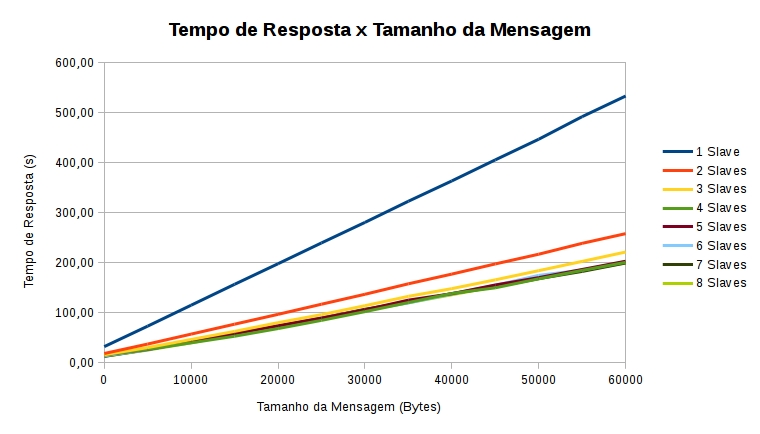
\includegraphics[scale=0.65]{figuras/temporesposta_centralizado.png}
\caption{Gráfico do Tempo de Resposta x Tamanho da Mensagem}
\label{fig:cent:tempo_respostaXtamanho_msg}
\end{figure}

A Figura \ref{fig:cent:speedupXtamanho_msg} apresenta o gráfico com o \textit{Speed Up} como função do tamanho da mensagem para diferentes números de escravos. Para se calcular o \textit{Speed Up} foi utilizado como tempo de execução serial o obtido pela aplicação centralizada.

Ao analisar o gráfico nota-se que à medida que o número de escravos aumenta o \textit{Speed Up} também vai aumentando, porém 
a partir de 4 escravos pra cima o seu valor varia muito pouco. Como visto em sala de aula verifica-se que o \textit{Speed Up}
obtido foi sublinear, o que era o esperado, pois segundo a Lei de Amdahl o maior \textit{Speed Up} que se consegue obter é o liner onde o \textit{Speed Up} é igual ao número de \textit{threads} de execução paralela, sendo que obter esse valor ótimo é
impossível visto que sempre existirá uma parte do programa que tem que ser executado serialmente, no caso desse trabalho o 
mestre é o que precisa executar algumas ações de forma serial.

\begin{figure}[!htb]
\centering
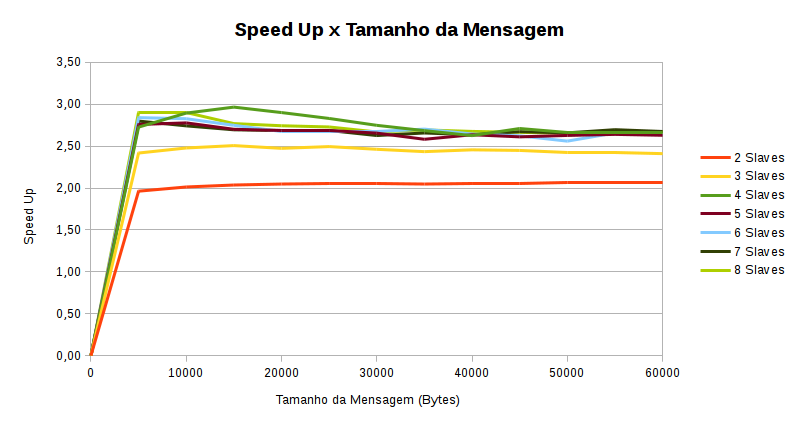
\includegraphics[scale=0.55]{figuras/speedup_centralizado.png}
\caption{Gráfico do Speed Up x Tamanho da Mensagem}
\label{fig:cent:speedupXtamanho_msg}
\end{figure}

A Figura \ref{fig:cent:eficienciaXtamanho_msg} apresenta o gráfico com a eficiência em função do tamanho da mensagem para 
diferentes números de escravos.

Ao observar o gráfico percebe-se claramente que quanto mais escravos são adicionados menor é a eficiência. Isso é esperado
visto que como observado na Figura \ref{fig:cent:speedupXtamanho_msg} à medida que aumenta-se o número de escravos o \textit{Speed Up} não se altera muito sendo o mesmo para mais do que 4 escravos com isso a eficiência tende a ser menor
para um número maior de escravos.

Um outro ponto a se destacar é que para 2 escravos e eficiência foi um pouco maior do que 1, isso é impossível pelo fato de
que a maior eficiência possível de se obter é 1. Isso pode ter ocorrido devido a ruídos que podem ter ocasionado em erros na
medição dos tempos.

\begin{figure}[!htb]
\centering
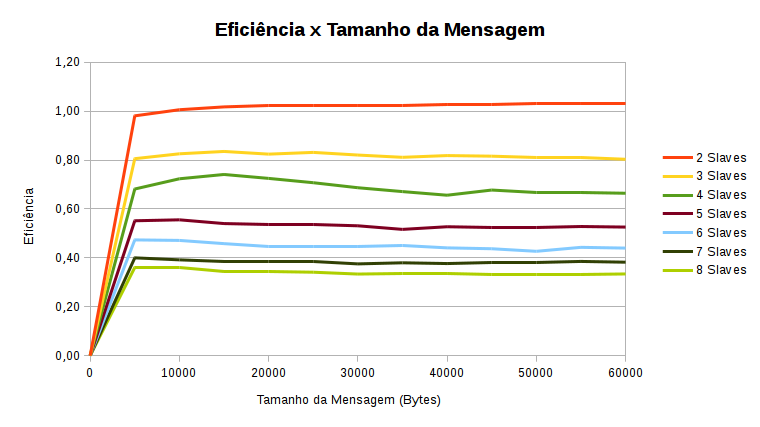
\includegraphics[scale=0.55]{figuras/eficiencia_centralizado.png}
\caption{Gráfico da Eficiência x Tamanho da Mensagem}
\label{fig:cent:eficienciaXtamanho_msg}
\end{figure}

Por fim, a Figura \ref{fig:cent:overheadXtamanho_msg} apresenta as medições do \textit{overhead} obtidos. Pode-se notar que 
o gráfico apresenta muita oscilação causada provavelmente por existirem processos do SO rodando em \textit{background}. Isso
faz com que não forneça informações tão relevantes, como os processos rodam na mesma máquina o \textit{overhead} é muito
pequeno sua medição acaba ficando refém dos ruídos.

\begin{figure}[!htb]
\centering
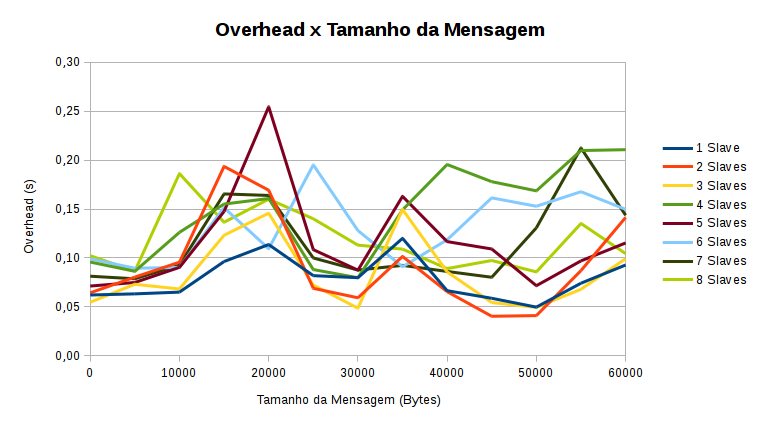
\includegraphics[scale=0.65]{figuras/overhead_centralizado.png}
\caption{Gráfico do Overhead x Tamanho da Mensagem}
\label{fig:cent:overheadXtamanho_msg}
\end{figure}


\section{Desempenho Distribuído em Várias Máquinas}

As medições para essa análise foram obtidas utilizando os computadores do LabGrad. Vale destacar que até os testes para a 
obtenção dos dados para 7 escravos o LabGrad estava com poucos alunos de graduação o que permitiu uma melhor medição dos tempos, porém ao se realizar a medição para 8 escravos, o LabGrad teve um problema de rede e quando foi resolvido haviam muitos alunos utilizando as máquinas, isso fez com que os dados obtidos para 8 escravos fossem prejudicados, porém mesmo com esse problema pode-se realizar uma análise do desempenho.

Para a medição dos dados também foi usada a aplicação cliente de teste para gerar tamanhos aleatórios de vetor de 0 a 60Kb,
sendo que os tamanhos foram espaçados de 5 em 5Kb.

Para os testes foram utilizados 4 máquinas. Para os testes até 4 escravos cada máquina possuía rodando apenas 1 escravo, para 5 escravos até 8 foram sendo adicionados escravos em cada uma dessas 4 máquinas de modo que ao final cada uma tivesse apenas 2
escravos rodando ao mesmo tempo. Essa estratégia foi usada pois cada computador possuía dois \textit{cores} de processamento.

A Figura \ref{fig:dist:tempo_respostaXtamanho_msg} apresenta um gráfico com o tempo de resposta obtido com diferentes tamanhos de mensagem para diferentes números de escravos de forma distribuída. Destaca-se que o caso onde existe apenas um escravo é a medição foi obtida com uma aplicação centralizada que realizou o ataque sozinha em uma das máquinas.

Ao observar o gráfico percebe-se claramente que à medida que aumenta-se o número de escravos, ou seja, faz-se a distribuição da tarefa entre as diferentes máquinas o tempo de resposta diminui como imaginado, como a tarefa será distribuída entre 
diferentes máquinas cada uma com uma pequena parte da tarefa espera-se que o processamento de cada parte seja mais rápido.
Destaca-se que o caso onde há apenas 1 escravo, foi medido rodando a mesma aplicação centralizada da análise anterior nas máquinas do LabGrad.

Uma observação interessante de se notar é que diferentemente do caso anterior onde se analisou o desempenho de paralelismo após a utilização de 4 escravos o tempo de resposta foi basicamente o mesmo para até 8 escravos. Já nesse caso distribuído 
nota-se que ao aumentar o número de escravos o tempo de resposta diminuiu para todos os escravos mesmo que a diferença entre 6 e 7 escravos seja pequena é possível observar uma diferença no tempo. Vale destacar novamente que para 8 escravos as medições foram prejudicadas pelo momento do teste e como não foi possível refazé-los eles apresentaram essa diferença. Mas acredita-se
que caso os problemas citados não tivessem ocorrido o grafíco apresentaria uma melhora mesmo que pequena no tempo de resposta
para o caso de 8 escravos.

\begin{figure}[!htb]
\centering
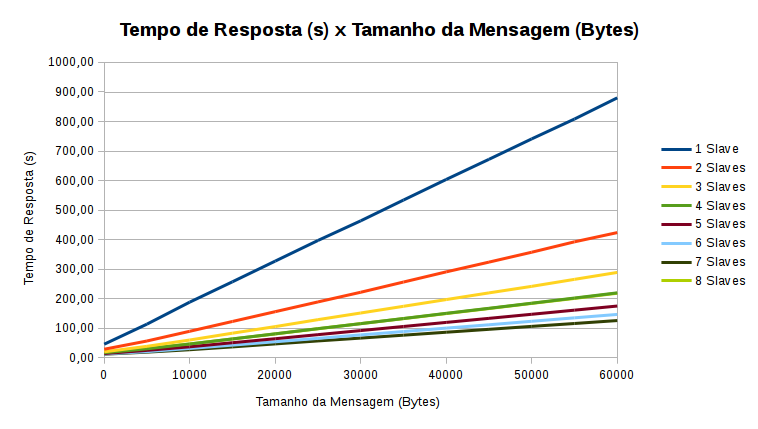
\includegraphics[scale=0.65]{figuras/temporesposta_distribuido.png}
\caption{Gráfico do Tempo de Resposta x Tamanho da Mensagem}
\label{fig:dist:tempo_respostaXtamanho_msg}
\end{figure}

A Figura \ref{fig:dist:speedupXtamanho_msg} apresenta o gráfico do \textit{Speed Up} em função do tamanho da mensagem para diferentes números de escravos. O tempo de execução serial utilizado para o cálculo foi o tempo de execução da aplicação centralizada nas máquinas do LabGrad.

Ao analisar o gráfico nota-se que à medida que o número de escravos aumenta o \textit{Speed Up} também vai aumentando, mas diferentemente da análise anterior eles não se aproximam de um valor em comum à medida que o número de escravos aumenta, sendo bem distintos. Para o caso de 8 escravos ele se equipara ao caso de 4 escravos devido aos problemas que ocorreram durante as medições. 

Como visto em sala de aula verifica-se que o \textit{Speed Up} obtido foi linear, o que inicialmente é estranho, já que 
esse é o máximo \textit{speed up} teórico possível.

Esse resultado pode ter sido obtido por alguns fatores:

\begin{itemize}
	\item Erros de medições dos tempos;
	\item O algoritmo sequencial não é o melhor que se pode conseguir;
	\item A lei de Amdahl considera que o caso serial é executado por um único processador, o que nesse caso não ocorre visto 
	que as máquinas possuem dois \textit{cores} de processamento, então mesmo que ela execute a tarefa sozinha o SO irá 
	dividi-lá entre os processadores.
\end{itemize}

\begin{figure}[!htb]
\centering
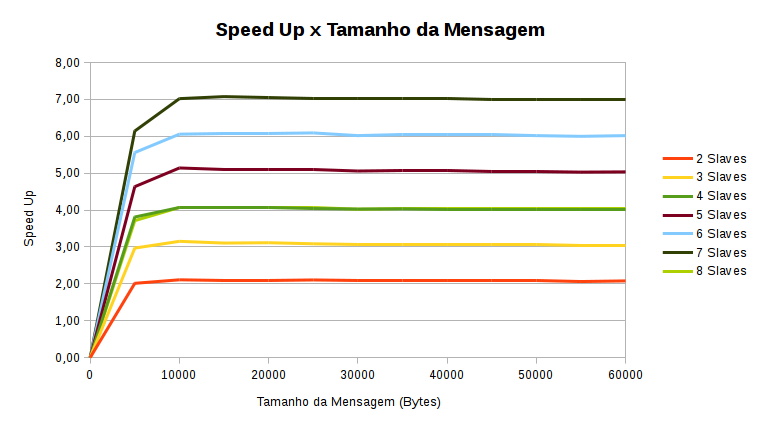
\includegraphics[scale=0.65]{figuras/speedup_distribuido.png}
\caption{Gráfico do Speed Up x Tamanho da Mensagem}
\label{fig:dist:speedupXtamanho_msg}
\end{figure}


A Figura \ref{fig:dist:eficienciaXtamanho_msg} apresenta a eficiência obtida para diferentes números de escravos. Percebe-se 
que a eficiência foi aproximadamente 1 para todos os casos, exceto para o de 8 escravos devido aos problemas já citados.

Percebe-se que a eficiência acaba oscilando para cima e para baixo de 1 isso pode ser ocasionado pelos mesmos problemas citados anteriormente para o \textit{Speed Up}. Com isso, considera-se aceitável os dados medidos já que eles não são muito
maiores do que o valor máximo possível que é 1.


\begin{figure}[!htb]
\centering
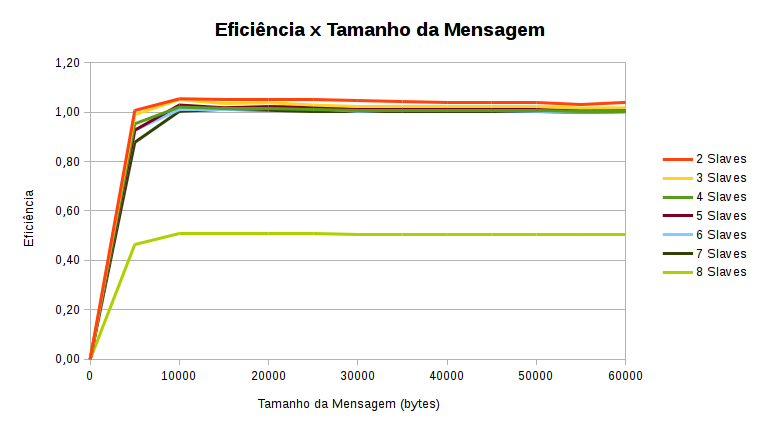
\includegraphics[scale=0.65]{figuras/eficiencia_distribuido.png}
\caption{Gráfico da Eficiência x Tamanho da Mensagem}
\label{fig:dist:eficienciaXtamanho_msg}
\end{figure}

A Figura \ref{fig:dist:overheadXtamanho_msg} apresenta o \textit{overhead} medido para diferentes números de escravos. 

Nesse caso observa-se uma oscilação ocasionada por ruídos da rede, mas mesmo com esse problema é possível verificar que à
medida que se aumenta o número de escravos o \textit{overhead} aumenta. O que é algo esperado visto que torna-se necessário 
enviar \textit{bytes} de dados para diferentes máquinas na rede.

\begin{figure}[!htb]
\centering
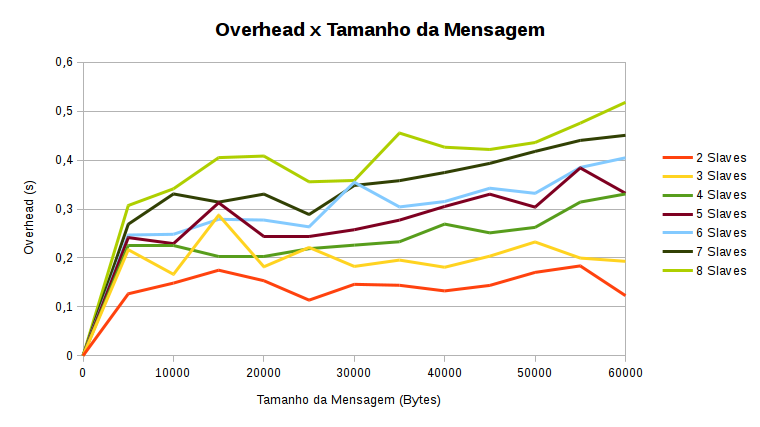
\includegraphics[scale=0.65]{figuras/overhead_distribuido.png}
\caption{Gráfico do Overhead x Tamanho da Mensagem}
\label{fig:dist:overheadXtamanho_msg}
\end{figure}

% Conclusão
% ---
\chapter{Conclusão}

Ao final desse trabalho é possível notar que um sistema distribuído é uma ferramenta muito poderosa pois permite aproveitar recursos de diferentes equipamentos para se executar uma tarefa em comum, de forma que com a distribuição do serviço entre as máquinas é consegue-se uma melhoria significativa no tempo de resposta. 

Através das análises realizadas foi possível verificar graficamente as vantagens de se realizar tarefas de forma paralela e/ou distribuída. Com essas análises também foi possível verificar alguns pontos interessantes, como o \textit{speed up} linear obtido na análise de desempenho distribuída, que é algo impossível de se obter e que pode ter sido causado pelos problemas citados, mas principalmente pelo fato de que a Lei de Amdahl considera o caso serial como sendo executado por um único processador, o que não ocorreu nesses casos visto que as máquinas possuíam mais de um \textit{core} de processamento.

Outro ponto importante e que foi possível notar durante a implementação desse trabalho é a complexidade de funcionamento que existe na máquina responsável por realizar todo o gerenciamento, nesse caso representada pelo mestre. Ele tem que lidar: com o controle de máquinas ativas, com a distribuição das tarefas, com o controle do status das tarefas, com o controle de concorrência, redistribuição de tarefas, entre outros. Além de todas essas tarefas ele ainda tem que cuidar do acesso
concorrente à variáveis de controle, que é um grande problema ao se trabalhar com muitas \textit{threads}, assim, percebe-se a necessidade que sempre vai existir para que algum pedaço do programa não seja paralelizável.


% ----------------------------------------------------------
% ELEMENTOS PÓS-TEXTUAIS
% ----------------------------------------------------------
\postextual


% ----------------------------------------------------------
% Referências bibliográficas
% ----------------------------------------------------------
%\bibliography{referencias} %% REFERENCIA AO ARQUIVO .bib

\end{document}
\grid
